Para no sobrecargar la parte anal\'itica del informe, en esta 
secci\'on vamos a acotar nuestro estudio a tres familias.

\subsubsection{Grafos bipartitos completos}

Sabemos del an\'alisis hecho anteriormente que la $CMF$ en un
grafo bipartito tiene a lo sumo dos nodos 
(ver secci\'on \ref{subsub:bipartitos}).
A grandes rasgos la busqueda tabu empezar\'a por cualquiera
de los nodos de una partici\'on, en particular la partici\'on
con menor cardinal, ya que si llamamos $\Delta_1$ al grado 
de cada uno de estos nodos (llamemos $A$ a la partici\'on formada
por los mismos) y $\Delta_2$ al grado de los nodos
en la partici\'on contraria ($B$), se verifica que:
\[ \text{\#nodos($A$)}= \Delta_2 \]
\[ \text{\#nodos($B$)}= \Delta_1 \]
\[ \forall v \in A: d(v)= \Delta_1 \]
\[ \forall u \in B: d(u)= \Delta_2 \]

Tambi\'en sabemos que la cantidad de aristas del grafo es:
\[ m = \Delta_1 \times \Delta_2 \]

Con esto el grado promedio ser\'a:
\[ \overline{d(v)} = \frac{2m}{n} = \frac{2 \Delta_1 \Delta_2}
{\Delta_1 + \Delta_2} \geq \frac{2 \Delta_1 \Delta_2}{2 \Delta1} 
= \Delta_2 \]
En virtud de que
\[ \Delta_1 \geq \Delta_2 \]
\[ \Delta_1 + \Delta_1 \geq \Delta_2 + \Delta_1 \]
\[ 2 \Delta_1 \geq \Delta_1 + \Delta_2 \]
O sea
\[ \overline{d(v)} \geq \Delta_2 \]

Con lo cual la heur\'istica s\'olo seleccionar\'a como 
punto de partida alguno de los nodos cuyo grado es $\Delta_1$, 
o sea un nodo de $A$. Como ya mencionamos, la soluci\'on ser\'a
la \'optima como tambi\'en lo era para las heur\'isticas golosa
y busqueda local, pero en este caso, dependiendo de los 
parametros de la busqueda tabu, puede llegar a tomar mayor 
tiempo de ejecuci\'on que las heur\'isticas alternativas.

Particularmente, para este caso la soluci\'on \'optima se 
obtendr\'a en a lo sumo 2 iteraciones. Si es muy alta la
cantidad de iteraciones sin mejorar que se permite, se 
puede pasar por todas las soluciones \'optimas repetidas 
veces.

Incluso siendo limitado este par\'ametro, en una implementaci\'on
gen\'erica, el hecho de que esto es lo que actua como una especie
de buffer para evitar estancarnos en un extremo local, 
lo fuerza a ser relativamente
grande, de lo contrario pierde su utilidad. Por esto para esta familia
muy limitada de grafos es m\'as conveniente aplicar cualquiera de las
otras heur\'isticas que la de busqueda tabu. Por supuesto verificar 
que un grafo corresponde a exactamente esta familia, no es una
tarea trivial.

\subsubsection{Estrella Doble}
Esta novedosa familia es en realidad producto de una relajaci\'on 
extrema de alguna de las condiciones de la familia \emph{Estrella
+ Puente + $CMF$} y a posteriori de una tensi\'on extrema de
otras condiciones en la familia resultante, quedando una familia
mucho m\'as r\'igida que la de partida, pero de esta manera m\'as
f\'acilmente analizable y cuyas conclusiones pueden ser generalizadas
a la familia de partida.

Descriptivamente se trata de una Estrella unida con un Puente simple
a una clique de dos nodos que es la $CMF$ del grafo, la peculiaridad
adicional de esta clique es que cada subgrafo inducido por uno de
los nodos de la clique y todos sus nodos adyacentes, es a su vez 
una estrella. En un principio no se impone ninguna condici\'on sobre
el puente, excepto que sea un camino simple uniendo la estrella 
solitaria y la clique de longitud mayor a tres (tomando desde la 
punta de la estrella hasta la punta m\'as cercana de la clique).


Sin entrar en mayor lujo de detalles, pasamos a exponer un ejemplo
\begin{center}
	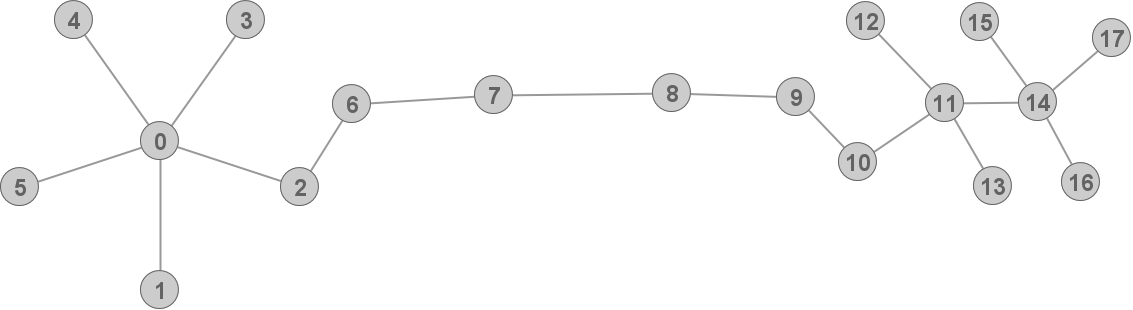
\includegraphics[scale = 0.3]{img/ej3/tabu_search/dobleEstrella_st0.png}
\end{center}

Aqu\'i por supuesto se ve que la estrella solitaria es el subgrafo 
inducido por los nodos $0$ a $5$, el puente el subgrafo inducido 
por los nodos $2$ y $6$ a $10$ y la $CMF$ el subgrafo inducido por
los nodos $11$ y $14$.

Que la heur\'istica de busqueda tab\'u llegue a la soluci\'on \'optima
o devuelva una soluci\'on sub-\'optima s\'olo depende, en esta
caracterizaci\'on, de la longitud del puente en relaci\'on con la 
cantidad de iteraciones sin mejorar y del factor del punto de 
partida. 
Notes\'e que si se empieza en alguno de los nodos de la 
clique o de los adyacentes a la misma, la soluci\'on \'optima
se encuentra en a lo sumo dos iteraciones, amen de la cantidad
de iteraciones sin mejorar que est\'e permitida. Como esta soluci\'on
nunca va a mejorar, cuando se termine la busqueda tab\'u devolver\'a
la $CMF$.
Por el contrario si la heur\'istica comienza a armar la soluci\'on
en la estrella solitaria o en alg\'un nodo del puente no adyacente 
a la clique, la heur\'istica puede no llegar nunca a considerar 
a la $CMF$ como soluci\'on (cuando se agotan la cantidad de 
iteraciones permitidas). Aqu\'i es donde se pone de manifiesto 
que el par\'ametro \emph{ cantidad de iteraciones sin mejorar} 
es central para grafos pertenecientes a esta familia o an\'alogos.

En este punto es donde se puede generalizar y concluir que los 
grafos de la familia \emph{Estrella + Puente + CMF} se comportan
de igual manera que lo hasta aqu\'i estudiado, ya que la limitaci\'on
respecto de esta heuristica que, determina la optimalidad del resultado
es en todos los casos la misma, la longitud del puente en relaci\'on
con la cantidad de iteraciones permitidas.

Veamos para concluir esta secci\'on 3 posibles soluciones (muy minimales)
arrojadas por la busqueda tab\'u para el grafo de ejemplo (para no 
sobrecargar el informe, se ver\'a solo el resultado obtenido).

Con el tama\~no del puente mayor a dos veces la cantidad de iteraciones
permitidas se arriba a los resultados mostrados, dependiendo del nodo
de inicio para la soluci\'on


\begin{center}
\begin{tabular}{|c||c|}
	\hline
	Nodo de comienzo & Soluci\'on busqueda tab\'u \\
	\hline
	\hline
	En la estrella &
	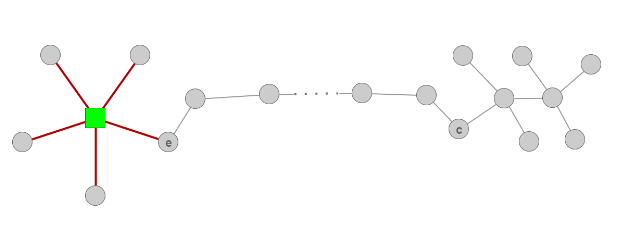
\includegraphics[scale = 0.5]{img/ej3/tabu_search/dobleEstrella_st11.png} \\
	\hline
	En nodo central del puente &
	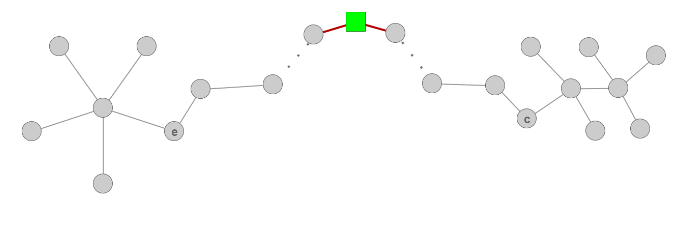
\includegraphics[scale = 0.5]{img/ej3/tabu_search/dobleEstrella_st21.png} \\
	\hline
	En la $CMF$ &
	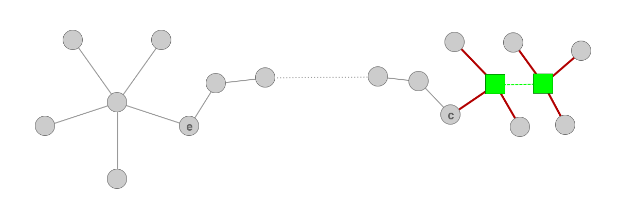
\includegraphics[scale = 0.5]{img/ej3/tabu_search/dobleEstrella_st01.png} \\
	\hline
\end{tabular}
\end{center}
